\documentclass{article}\usepackage[]{graphicx}\usepackage[]{color}
%% maxwidth is the original width if it is less than linewidth
%% otherwise use linewidth (to make sure the graphics do not exceed the margin)
\makeatletter
\def\maxwidth{ %
  \ifdim\Gin@nat@width>\linewidth
    \linewidth
  \else
    \Gin@nat@width
  \fi
}
\makeatother

\definecolor{fgcolor}{rgb}{0.345, 0.345, 0.345}
\newcommand{\hlnum}[1]{\textcolor[rgb]{0.686,0.059,0.569}{#1}}%
\newcommand{\hlstr}[1]{\textcolor[rgb]{0.192,0.494,0.8}{#1}}%
\newcommand{\hlcom}[1]{\textcolor[rgb]{0.678,0.584,0.686}{\textit{#1}}}%
\newcommand{\hlopt}[1]{\textcolor[rgb]{0,0,0}{#1}}%
\newcommand{\hlstd}[1]{\textcolor[rgb]{0.345,0.345,0.345}{#1}}%
\newcommand{\hlkwa}[1]{\textcolor[rgb]{0.161,0.373,0.58}{\textbf{#1}}}%
\newcommand{\hlkwb}[1]{\textcolor[rgb]{0.69,0.353,0.396}{#1}}%
\newcommand{\hlkwc}[1]{\textcolor[rgb]{0.333,0.667,0.333}{#1}}%
\newcommand{\hlkwd}[1]{\textcolor[rgb]{0.737,0.353,0.396}{\textbf{#1}}}%
\let\hlipl\hlkwb

\usepackage{framed}
\makeatletter
\newenvironment{kframe}{%
 \def\at@end@of@kframe{}%
 \ifinner\ifhmode%
  \def\at@end@of@kframe{\end{minipage}}%
  \begin{minipage}{\columnwidth}%
 \fi\fi%
 \def\FrameCommand##1{\hskip\@totalleftmargin \hskip-\fboxsep
 \colorbox{shadecolor}{##1}\hskip-\fboxsep
     % There is no \\@totalrightmargin, so:
     \hskip-\linewidth \hskip-\@totalleftmargin \hskip\columnwidth}%
 \MakeFramed {\advance\hsize-\width
   \@totalleftmargin\z@ \linewidth\hsize
   \@setminipage}}%
 {\par\unskip\endMakeFramed%
 \at@end@of@kframe}
\makeatother

\definecolor{shadecolor}{rgb}{.97, .97, .97}
\definecolor{messagecolor}{rgb}{0, 0, 0}
\definecolor{warningcolor}{rgb}{1, 0, 1}
\definecolor{errorcolor}{rgb}{1, 0, 0}
\newenvironment{knitrout}{}{} % an empty environment to be redefined in TeX

\usepackage{alltt}
\usepackage{Sweave}
\usepackage{float}
\usepackage{graphicx}
\usepackage{tabularx}
\usepackage{siunitx}
\usepackage{mdframed}
\usepackage{amsmath}
\usepackage{gensymb}
\usepackage{natbib}
\bibliographystyle{..//refs/styles/besjournals.bst}
\usepackage[small]{caption}
\setkeys{Gin}{width=0.8\textwidth}
\setlength{\captionmargin}{30pt}
\setlength{\abovecaptionskip}{0pt}
\setlength{\belowcaptionskip}{10pt}
\topmargin -1.5cm        
\oddsidemargin -0.04cm   
\evensidemargin -0.04cm
\textwidth 16.59cm
\textheight 21.94cm 
%\pagestyle{empty} %comment if want page numbers
\parskip 7.2pt
\renewcommand{\baselinestretch}{1.5}
\parindent 0pt

\newmdenv[
  topline=true,
  bottomline=true,
  skipabove=\topsep,
  skipbelow=\topsep
]{siderules}

%% R Script


\IfFileExists{upquote.sty}{\usepackage{upquote}}{}
\begin{document}

\renewcommand{\thetable}{\arabic{table}}
\renewcommand{\thefigure}{\arabic{figure}}
\renewcommand{\labelitemi}{$-$}
%%%%%%%%%%%%%%%%%%%%%%%%%%%%%%%%%%%%%%%%%%%%%%%%%%%%%%%%%%%%%%%%%%%%%%%%%%%%%%%%%%%%%%%%%%%
\section*{Chilling Experiment Figures}

\begin{figure} [H]
\begin{center}
\caption{Day of budburst and the day of leaf out for native tree species in New England. Data was collected from a growth chamber experiment using any combination of two photoperiod treatments, two forcing treatments, and three chilling treatments. The standard deviation is represented in blue for budburst and green for leaf out. }
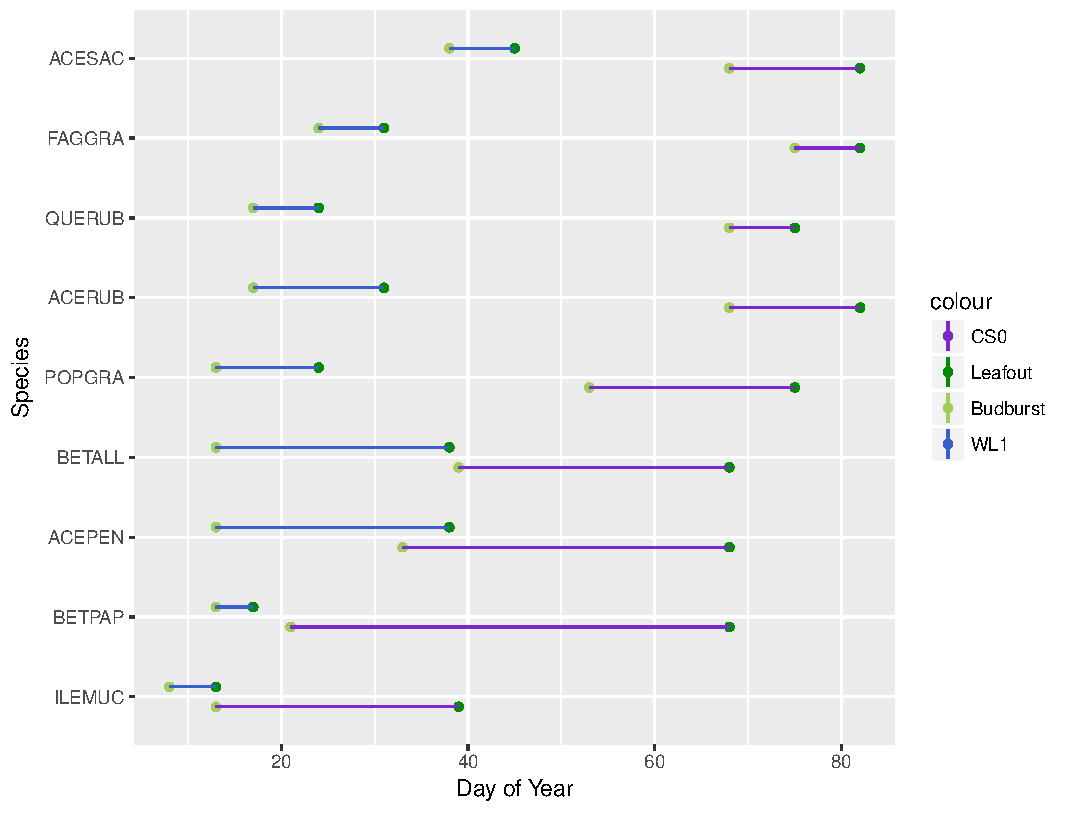
\includegraphics{..//figure/Exp_plot.pdf} 
\end{center}
\end{figure}

\begin{figure}[H]
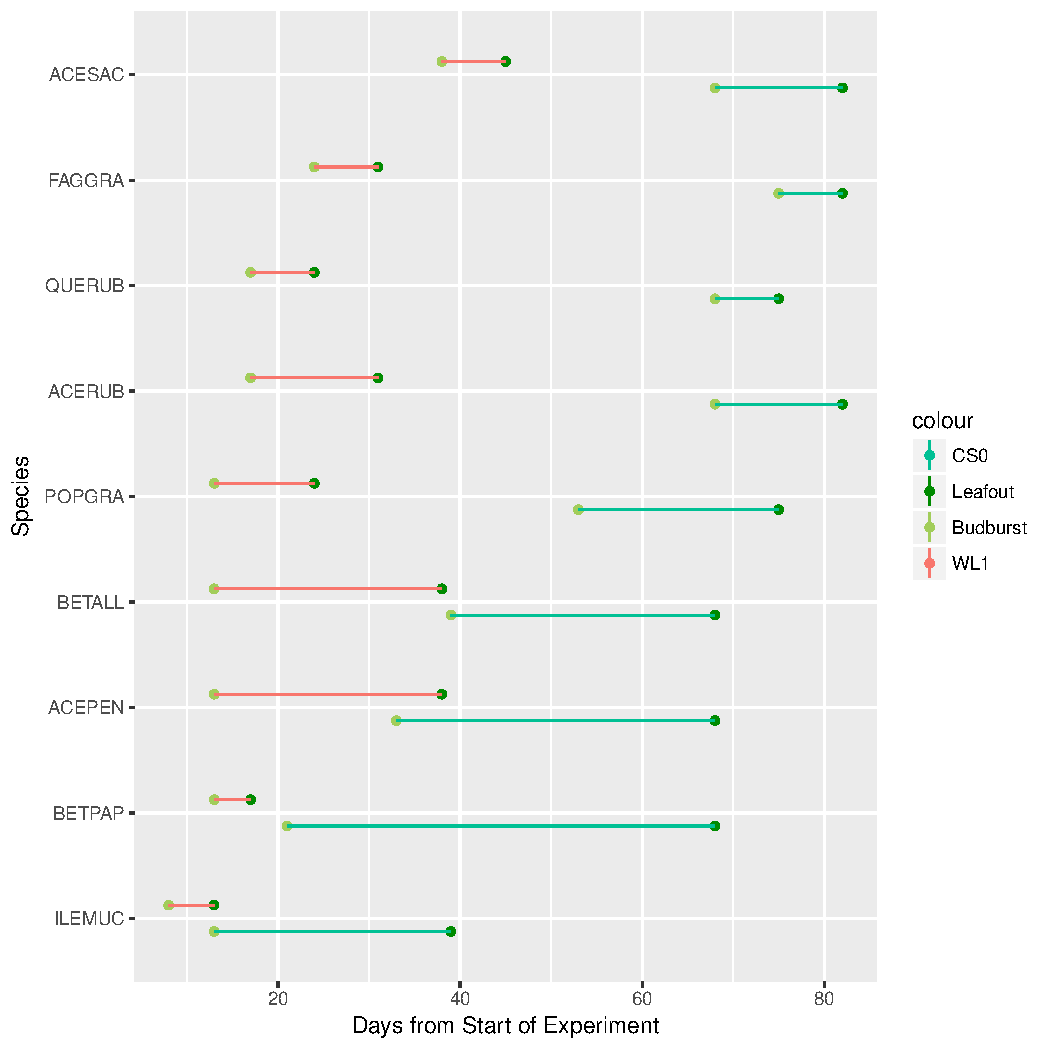
\includegraphics[width=\maxwidth]{figure/dan-1} \caption[A scatterplot indicating FSI values from 2008 to 2014 for each methdology used in this study]{A scatterplot indicating FSI values from 2008 to 2014 for each methdology used in this study. PhenoCam FSI values are red, Observed FSI values are blue, and USA-NPN FSI values are green.}\label{fig:dan}
\end{figure}





% latex table generated in R 3.3.1 by xtable 1.8-2 package
% Thu Jun  8 08:22:22 2017
\begin{table}[ht]
\centering
\begin{tabular}{rrrrr}
  \hline
  ACEPEN & Sum.Sq & Df & F value & Pr(>F) \\
 \hline
chilling & 149.41 &   2 & 1.20 & 0.30 \\ 
  forcing & 4909.59 &   1 & 78.94 & 0.00 \\ 
  photoperiod & 1309.59 &   1 & 21.06 & 0.00 \\ 
  Residuals & 6654.56 & 107 &  &  \\ 
   \hline
\end{tabular}
\end{table}
% latex table generated in R 3.3.1 by xtable 1.8-2 package
% Thu Jun  8 08:22:22 2017
\begin{table}[ht]
\centering
\begin{tabular}{rrrrr}
  \hline
  ACERUB & Sum.Sq & Df & F value & Pr(>F) \\
 \hline
chilling & 0.62 &   2 & 0.00 & 1.00 \\ 
  forcing & 1731.00 &   1 & 25.92 & 0.00 \\ 
  photoperiod & 462.78 &   1 & 6.93 & 0.01 \\ 
  Residuals & 6611.17 &  99 &  &  \\ 
   \hline
\end{tabular}
\end{table}
% latex table generated in R 3.3.1 by xtable 1.8-2 package
% Thu Jun  8 08:22:22 2017
\begin{table}[ht]
\centering
\begin{tabular}{rrrrr}
  \hline
  ACESAC & Sum.Sq & Df & F value & Pr(>F) \\
 \hline
chilling & 65.41 &   2 & 0.46 & 0.64 \\ 
  forcing & 259.14 &   1 & 3.61 & 0.06 \\ 
  photoperiod & 231.41 &   1 & 3.22 & 0.08 \\ 
  Residuals & 4524.88 &  63 &  &  \\ 
   \hline
\end{tabular}
\end{table}
% latex table generated in R 3.3.1 by xtable 1.8-2 package
% Thu Jun  8 08:22:22 2017
\begin{table}[ht]
\centering
\begin{tabular}{rrrrr}
  \hline
  BETALL & Sum.Sq & Df & F value & Pr(>F) \\
 \hline
chilling & 525.95 &   2 & 5.00 & 0.01 \\ 
  forcing & 1463.30 &   1 & 27.81 & 0.00 \\ 
  photoperiod & 632.83 &   1 & 12.03 & 0.00 \\ 
  Residuals & 6944.50 & 132 &  &  \\ 
   \hline
\end{tabular}
\end{table}
% latex table generated in R 3.3.1 by xtable 1.8-2 package
% Thu Jun  8 08:22:22 2017
\begin{table}[ht]
\centering
\begin{tabular}{rrrrr}
  \hline
  BETPAP & Sum.Sq & Df & F value & Pr(>F) \\
 \hline
chilling & 6.00 &   2 & 0.04 & 0.96 \\ 
  forcing & 1776.23 &   1 & 21.47 & 0.00 \\ 
  photoperiod & 1105.08 &   1 & 13.35 & 0.00 \\ 
  Residuals & 10509.00 & 127 &  &  \\ 
   \hline
\end{tabular}
\end{table}
% latex table generated in R 3.3.1 by xtable 1.8-2 package
% Thu Jun  8 08:22:22 2017
\begin{table}[ht]
\centering
\begin{tabular}{rrrrr}
  \hline
  FAGGRA & Sum.Sq & Df & F value & Pr(>F) \\
 \hline
chilling & 144.41 &   2 & 1.66 & 0.20 \\ 
  forcing & 611.20 &   1 & 14.04 & 0.00 \\ 
  photoperiod & 1.05 &   1 & 0.02 & 0.88 \\ 
  Residuals & 2829.78 &  65 &  &  \\ 
   \hline
\end{tabular}
\end{table}
% latex table generated in R 3.3.1 by xtable 1.8-2 package
% Thu Jun  8 08:22:22 2017
\begin{table}[ht]
\centering
\begin{tabular}{rrrrr}
  \hline
  ILEMUC & Sum.Sq & Df & F value & Pr(>F) \\
 \hline
chilling & 26.49 &   2 & 0.54 & 0.59 \\ 
  forcing & 2262.34 &   1 & 91.61 & 0.00 \\ 
  photoperiod & 1035.85 &   1 & 41.94 & 0.00 \\ 
  Residuals & 3334.05 & 135 &  &  \\ 
   \hline
\end{tabular}
\end{table}
% latex table generated in R 3.3.1 by xtable 1.8-2 package
% Thu Jun  8 08:22:23 2017
\begin{table}[ht]
\centering
\begin{tabular}{rrrrr}
  \hline
  POPGRA & Sum.Sq & Df & F value & Pr(>F) \\
 \hline
chilling & 54.63 &   2 & 0.39 & 0.68 \\ 
  forcing & 2405.73 &   1 & 34.52 & 0.00 \\ 
  photoperiod & 1019.78 &   1 & 14.63 & 0.00 \\ 
  Residuals & 6760.98 &  97 &  &  \\ 
   \hline
\end{tabular}
\end{table}
% latex table generated in R 3.3.1 by xtable 1.8-2 package
% Thu Jun  8 08:22:23 2017
\begin{table}[ht]
\centering
\begin{tabular}{rrrrr}
  \hline
  QUERUB & Sum.Sq & Df & F value & Pr(>F) \\
 \hline
chilling & 35.61 &   2 & 0.45 & 0.64 \\ 
  forcing & 680.83 &   1 & 17.34 & 0.00 \\ 
  photoperiod & 369.53 &   1 & 9.41 & 0.00 \\ 
  Residuals & 4946.29 & 126 &  &  \\ 
   \hline
\end{tabular}
\end{table}


% latex table generated in R 3.3.1 by xtable 1.8-2 package
% Thu Jun  8 08:22:23 2017
\begin{table}[ht]
\centering
\begin{tabular}{rrrrr}
  \hline
  ACEPEN & Sum.Sq & Df & F value & Pr(>F) \\
 \hline
chilling & 104.66 &   2 & 0.87 & 0.42 \\ 
  forcing & 4745.38 &   1 & 79.18 & 0.00 \\ 
  photoperiod & 1306.03 &   1 & 21.79 & 0.00 \\ 
  chilling:forcing & 63.31 &   2 & 0.53 & 0.59 \\ 
  chilling:photoperiod & 181.96 &   2 & 1.52 & 0.22 \\ 
  forcing:photoperiod & 257.63 &   1 & 4.30 & 0.04 \\ 
  Residuals & 6113.18 & 102 &  &  \\ 
   \hline
\end{tabular}
\end{table}
% latex table generated in R 3.3.1 by xtable 1.8-2 package
% Thu Jun  8 08:22:23 2017
\begin{table}[ht]
\centering
\begin{tabular}{rrrrr}
  \hline
  ACERUB & Sum.Sq & Df & F value & Pr(>F) \\
 \hline
chilling & 1.53 &   2 & 0.01 & 0.99 \\ 
  forcing & 1721.25 &   1 & 26.13 & 0.00 \\ 
  photoperiod & 381.81 &   1 & 5.80 & 0.02 \\ 
  chilling:forcing & 358.58 &   2 & 2.72 & 0.07 \\ 
  chilling:photoperiod & 37.69 &   2 & 0.29 & 0.75 \\ 
  forcing:photoperiod & 17.35 &   1 & 0.26 & 0.61 \\ 
  Residuals & 6191.98 &  94 &  &  \\ 
   \hline
\end{tabular}
\end{table}
% latex table generated in R 3.3.1 by xtable 1.8-2 package
% Thu Jun  8 08:22:23 2017
\begin{table}[ht]
\centering
\begin{tabular}{rrrrr}
  \hline
  ACESAC & Sum.Sq & Df & F value & Pr(>F) \\
 \hline
chilling & 65.78 &   2 & 0.45 & 0.64 \\ 
  forcing & 204.31 &   1 & 2.83 & 0.10 \\ 
  photoperiod & 267.24 &   1 & 3.70 & 0.06 \\ 
  chilling:forcing & 76.27 &   2 & 0.53 & 0.59 \\ 
  chilling:photoperiod & 164.28 &   2 & 1.14 & 0.33 \\ 
  forcing:photoperiod & 0.05 &   1 & 0.00 & 0.98 \\ 
  Residuals & 4194.28 &  58 &  &  \\ 
   \hline
\end{tabular}
\end{table}
% latex table generated in R 3.3.1 by xtable 1.8-2 package
% Thu Jun  8 08:22:23 2017
\begin{table}[ht]
\centering
\begin{tabular}{rrrrr}
  \hline
  BETALL & Sum.Sq & Df & F value & Pr(>F) \\
 \hline
chilling & 526.41 &   2 & 5.57 & 0.00 \\ 
  forcing & 1463.33 &   1 & 30.95 & 0.00 \\ 
  photoperiod & 632.83 &   1 & 13.38 & 0.00 \\ 
  chilling:forcing & 66.32 &   2 & 0.70 & 0.50 \\ 
  chilling:photoperiod & 226.18 &   2 & 2.39 & 0.10 \\ 
  forcing:photoperiod & 612.56 &   1 & 12.95 & 0.00 \\ 
  Residuals & 6005.50 & 127 &  &  \\ 
   \hline
\end{tabular}
\end{table}
% latex table generated in R 3.3.1 by xtable 1.8-2 package
% Thu Jun  8 08:22:23 2017
\begin{table}[ht]
\centering
\begin{tabular}{rrrrr}
  \hline
  BETPAP & Sum.Sq & Df & F value & Pr(>F) \\
 \hline
chilling & 6.07 &   2 & 0.04 & 0.96 \\ 
  forcing & 1765.57 &   1 & 21.22 & 0.00 \\ 
  photoperiod & 1101.18 &   1 & 13.24 & 0.00 \\ 
  chilling:forcing & 71.38 &   2 & 0.43 & 0.65 \\ 
  chilling:photoperiod & 62.92 &   2 & 0.38 & 0.69 \\ 
  forcing:photoperiod & 233.62 &   1 & 2.81 & 0.10 \\ 
  Residuals & 10148.80 & 122 &  &  \\ 
   \hline
\end{tabular}
\end{table}
% latex table generated in R 3.3.1 by xtable 1.8-2 package
% Thu Jun  8 08:22:23 2017
\begin{table}[ht]
\centering
\begin{tabular}{rrrrr}
  \hline
  FAGGRA & Sum.Sq & Df & F value & Pr(>F) \\
 \hline
chilling & 145.37 &   2 & 1.64 & 0.20 \\ 
  forcing & 595.26 &   1 & 13.40 & 0.00 \\ 
  photoperiod & 0.42 &   1 & 0.01 & 0.92 \\ 
  chilling:forcing & 39.45 &   2 & 0.44 & 0.64 \\ 
  chilling:photoperiod & 83.56 &   2 & 0.94 & 0.40 \\ 
  forcing:photoperiod & 35.33 &   1 & 0.80 & 0.38 \\ 
  Residuals & 2665.38 &  60 &  &  \\ 
   \hline
\end{tabular}
\end{table}
% latex table generated in R 3.3.1 by xtable 1.8-2 package
% Thu Jun  8 08:22:23 2017
\begin{table}[ht]
\centering
\begin{tabular}{rrrrr}
  \hline
  ILEMUC & Sum.Sq & Df & F value & Pr(>F) \\
 \hline
chilling & 28.03 &   2 & 0.60 & 0.55 \\ 
  forcing & 2277.73 &   1 & 97.37 & 0.00 \\ 
  photoperiod & 1033.49 &   1 & 44.18 & 0.00 \\ 
  chilling:forcing & 16.09 &   2 & 0.34 & 0.71 \\ 
  chilling:photoperiod & 106.28 &   2 & 2.27 & 0.11 \\ 
  forcing:photoperiod & 171.89 &   1 & 7.35 & 0.01 \\ 
  Residuals & 3041.00 & 130 &  &  \\ 
   \hline
\end{tabular}
\end{table}
% latex table generated in R 3.3.1 by xtable 1.8-2 package
% Thu Jun  8 08:22:23 2017
\begin{table}[ht]
\centering
\begin{tabular}{rrrrr}
  \hline
  POPGRA & Sum.Sq & Df & F value & Pr(>F) \\
 \hline
chilling & 50.56 &   2 & 0.37 & 0.69 \\ 
  forcing & 2390.66 &   1 & 35.16 & 0.00 \\ 
  photoperiod & 1016.39 &   1 & 14.95 & 0.00 \\ 
  chilling:forcing & 45.72 &   2 & 0.34 & 0.72 \\ 
  chilling:photoperiod & 152.02 &   2 & 1.12 & 0.33 \\ 
  forcing:photoperiod & 296.37 &   1 & 4.36 & 0.04 \\ 
  Residuals & 6254.69 &  92 &  &  \\ 
   \hline
\end{tabular}
\end{table}
% latex table generated in R 3.3.1 by xtable 1.8-2 package
% Thu Jun  8 08:22:23 2017
\begin{table}[ht]
\centering
\begin{tabular}{rrrrr}
  \hline
  QUERUB & Sum.Sq & Df & F value & Pr(>F) \\
 \hline
chilling & 35.70 &   2 & 0.46 & 0.63 \\ 
  forcing & 668.59 &   1 & 17.39 & 0.00 \\ 
  photoperiod & 364.39 &   1 & 9.48 & 0.00 \\ 
  chilling:forcing & 174.11 &   2 & 2.26 & 0.11 \\ 
  chilling:photoperiod & 110.91 &   2 & 1.44 & 0.24 \\ 
  forcing:photoperiod & 15.92 &   1 & 0.41 & 0.52 \\ 
  Residuals & 4652.62 & 121 &  &  \\ 
   \hline
\end{tabular}
\end{table}


\end{document}
